%!TEX root = TheCourse.tex

\part{Continuous Probability Distributions}

\only<presentation>{\againframe{RecapDescriptiveStatistics}

\begin{frame}{Recap: Probability Fundamentals}
We moved from descriptive statistics to predicting the future using probability.
    
    \vspace{0.2cm}
    \begin{itemize}
        \item \textbf{The Addition Law (Unions):} When finding the probability of event $A$ OR event $B$, we add their probabilities but must subtract the intersection to avoid counting it twice
        $$P(A \cup B) = P(A) + P(B) - P(A \cap B)$$
        
        \vspace{0.2cm}
        \item \textbf{The Multiplication Law (Intersections):} When finding the probability of $A$ AND $B$, we use conditional probability to account for dependent events
        $$P(A \cap B) = P(A) \times P(B|A)$$ 
    \end{itemize}
\end{frame}

\begin{frame}{Recap: Discrete Distributions}
    We then mapped these events to numerical values, known as Discrete Random Variables 
    
    \vspace{0.2cm}
    \begin{itemize}
        \item \textbf{Expected Value:} The long-run average, $E(X) = \sum xP(x)$ 
        
        \vspace{0.2cm}
        \item \textbf{The Binomial Model:} Models successes in a fixed number of independent trials ($n$) with binary outcomes.
        \begin{itemize}
            \item Mean: $\mu = np$
        \end{itemize}
        
        \vspace{0.2cm}
        \item \textbf{The Poisson Model:} Models rare events over a continuous interval (like time or space)
        \begin{itemize}
            \item The Mathematical Oddity: Mean and Variance are exactly equal ($\mu = \sigma^2 = \lambda$)
        \end{itemize}
    \end{itemize}
\end{frame}

\begin{frame}{Today: The Next Step}
    \begin{block}{The Big Question}
        The Binomial and Poisson models deal with countable, discrete things (e.g., $0, 1, 2, 3...$)
        
        \vspace{0.2cm}
        But what happens when our random variable is a \textbf{continuous physical measurement}? 
    \end{block}
    
    \vspace{0.5cm}
    \begin{center}
        \Large \textit{Welcome to Continuous Probability Distributions!}
    \end{center}
\end{frame}

}

\section{Continuous Random Variables}

\subsection{From Counting to Measuring}
\begin{frame}{From Counting to Measuring}
    So far, we have looked at \textbf{Discrete} variables: things we can count (e.g., $0, 1, 2$ defective chips). 
  \only<presentation>{  
    \vspace{0.2cm}}
    But what if we are measuring the exact voltage of a 5V power supply? It might be $5.01\text{V}$, or $5.013\text{V}$, or $5.01347\text{V}\dots$
    
    \begin{definition}[Continuous Random Variable]
        A continuous random variable can take on \textit{any} real value within a given range. Because there are infinitely many possible values, we cannot list them in a table or use a Probability Mass Function.
    \end{definition}

    \only<article>{
        \textbf{The Histogram Connection:} Imagine drawing a histogram of battery voltages. If you measure 10 batteries, your bins are wide and blocky. If you measure 10,000 batteries and make your bins infinitely narrow, the jagged top of the histogram smooths out into a continuous curve. This curve is the foundation of continuous probability!
    }
\end{frame}

\subsection{The Probability Density Function (PDF)}
\begin{frame}{The Probability Density Function (PDF)}
    \only<article>{Instead of a table, c}\only<presentation>{C}ontinuous variables are defined \only<article>{by a mathematical curve called }a \textbf{Probability Density Function}, or PDF, usually denoted as $f(x)$.

    \begin{block}{Two Rules of a PDF}
        \begin{enumerate}
            \item The curve must never dip below the x-axis: $f(x) \geq 0$.
            \item The \textbf{total area} under the entire curve must equal exactly 1 (or $100\%$).
        \end{enumerate}
    \end{block}

    \pause 
    \begin{alertblock}{The Golden Rule of Continuous Probability}
        \only<article>{In a continuous distribution, probability is equivalent to \textbf{Area}. \\}
        To find the probability that a value falls between $a$ and $b$, you calculate the area under the curve between those two points:
        \[ P(a \leq X \leq b) = \int_{a}^{b} f(x) \,dx \]
    \end{alertblock}
\end{frame}

\begin{frame}{The \lq Exact Point\rq\ Paradox}
    \begin{example}[The infinitely precise resistor]
        Suppose you have a resistor that is supposedly exactly $100\,\Omega$. What is the probability that its true, physical resistance is \textit{exactly} $100.000000000\dots\,\Omega$ with infinite precision?
    \end{example}

    \pause 
       \begin{solution}
        Mathematically, a single point has a width of zero. Therefore, the area under the curve at exactly one point is zero!
        \[ P(X = 100) = \int_{100}^{100} f(x) \,dx = \mathbf{0} \]
        
        \textbf{Engineering Takeaway:} For continuous variables, it is meaningless to ask for the probability of an \textit{exact} number. We can only ask for the probability that a value falls within a \textbf{tolerance range} (e.g., between $99.9\,\Omega$ and $100.1\,\Omega$).
    \end{solution}
\end{frame}

\begin{frame}{The Cumulative Distribution Function (CDF)}
  \only<article>{  Since the probability of measuring an exact point is zero, engineers usually ask a different question: \textit{\lq What is the probability that a measurement is less than or equal to a certain value?\rq}
    
    To answer this, we use the \textbf{Cumulative Distribution Function (CDF)}, denoted by a capital $F(x)$.}
    
    \begin{definition}[The CDF]
        The CDF gives the accumulated area under the PDF curve from negative infinity up to a specific point $x$:
        \[ F(x) = P(X \leq x) = \int_{-\infty}^{x} f(t) \,dt \]
    \end{definition}

    \pause \vspace{0.2cm}
    \begin{block}{Why the CDF is powerful}
        If you already know the CDF, finding the probability of a value falling within a range becomes simple subtraction, with no integration required!
        \[ P(a \leq X \leq b) = F(b) - F(a) \]
    \end{block}
    
    \only<article>{
        \vspace{0.2cm}
        \textbf{Engineering Intuition:} If $f(x)$ represents the exact rate at which components fail at time $x$, then $F(x)$ represents the total percentage of components that have failed \textit{up to} time $x$. Because probability accumulates, a CDF curve always starts at 0 (0\% probability) and steadily climbs until it levels off at 1 (100\% probability).
    }
\end{frame}

\begin{frame}{Mean and Variance of Continuous Distributions}
  \only<article>{  Just as we did for discrete distributions, we can find the centre and spread of a continuous probability density function (PDF). The summations ($\sum$) simply become integrals ($\int$) over the entire domain.}

    \begin{block}{Expected Value (Mean)}
        The expected value, $\mu$ or $E(X)$, represents the \lq centre-of-mass\rq\ of the distribution:
        \[ \mu = E(X) = \int_{-\infty}^{\infty} x f(x) \dd x \]
          \only<article>{Recall that for a discrete random variable, the expected value was the sum of each outcome multiplied by its probability:
        \[ E(X) = \sum x P(x). \]}
    \end{block}



    \pause    
    \begin{block}{Variance}
        The variance, $\sigma^2$ or $V(X)$, measures the spread around the mean:
        \[ \sigma^2 = V(X) = \int_{-\infty}^{\infty} (x - \mu)^2 f(x) \dd x \]
        
   \only<article>{     \textbf{The Shortcut Formula:} Just like the discrete case, it is usually much easier to calculate using $E(X^2)$:}
        \[ V(X) = E(X^2) - [E(X)]^2 \quad \text{where} \quad E(X^2) = \int_{-\infty}^{\infty} x^2 f(x) \dd x \]
    \end{block}
    
    \only<article>{
        \vspace{0.3cm}
        \textit{Note that standard deviation ($\sigma$) is still just the square root of the variance.}
    }
\end{frame}

\begin{frame}{Worked Example: A Custom Continuous Distribution}
    \begin{example}[Sensor Calibration Error]
        An engineer models the calibration error $X$ (in millivolts) of a new prototype thermal sensor using the following Probability Density Function (PDF):
        \[
        f(x) = \begin{cases} 
        cx & \text{for } 0 \leq x \leq 2 \\
        0 & \text{otherwise}
        \end{cases}
        \]
        
        \textbf{Questions:}
        \begin{enumerate}
            \item Find the constant $c$ that makes this a valid PDF.
            \item Determine the Cumulative Distribution Function (CDF), $F(x)$.
            \item What is the probability that the error is less than $1\text{ mV}$?
            \item Calculate the expected (mean) error, $E(X)$.
            \item Calculate the variance (spread).
        \end{enumerate}
    \end{example}
\end{frame}

\begin{frame}{Solution: A Custom Continuous Distribution (1/4)}
    \begin{solution}
        \textbf{1. Find the constant $c$:} \\
        The total area under the PDF must equal exactly 1.
        \begin{align*}
            \int_{0}^{2} cx \dd x &= 1 \\
            \left[ c \frac{x^2}{2} \right]_{0}^{2} &= 1 \\
            c \left( \frac{4}{2} - 0 \right) &= 1 \implies 2c = 1 \implies \mathbf{c = 0.5}
        \end{align*}
        So, our complete PDF is $f(x) = 0.5x$ (for $0 \leq x \leq 2$).
    \end{solution}
\end{frame}

\begin{frame}{Solution: A Custom Continuous Distribution (2/4)}
    \begin{solutioncont}
        \textbf{2. Determine the CDF, $F(x)$:} \\
        The CDF accumulates area from the lower bound ($0$) up to an arbitrary point $x$. We integrate using a dummy variable $t$:
        \begin{align*}
            F(x) &= \int_{0}^{x} 0.5t \dd t \\
                 &= \left[ 0.25 t^2 \right]_{0}^{x} = \mathbf{0.25 x^2}
        \end{align*}
        \textit{(Valid for $0 \leq x \leq 2$. Once $x$ passes 2, the CDF stays flat at 1).}
    \end{solutioncont}
\end{frame}

\begin{frame}{Solution: A Custom Continuous Distribution (3/4)}
    \begin{solutioncont}
        \textbf{3. Probability the error is less than $1\text{ mV}$ ($P(X < 1)$):} \\
        Because we already found the CDF, we don't need to integrate again! We simply plug $1$ into $F(x)$:
        \[ P(X < 1) = F(1) = 0.25(1)^2 = \mathbf{0.25} \text{ \textbf{(or 25\%)}} \]
    \end{solutioncont}
\end{frame}

\begin{frame}{Solution: A Custom Continuous Distribution (4/4)}
    \begin{solutioncont}
        \textbf{4. Expected Value (Mean), $E(X)$:} \\
        For continuous variables, the sum becomes an integral: $E(X) = \int x f(x) \dd x$.
        \begin{align*}
            E(X) &= \int_{0}^{2} x (0.5x) \dd x \\
                 &= \int_{0}^{2} 0.5x^2 \dd x \\
                 &= \left[ \frac{0.5x^3}{3} \right]_{0}^{2} = \frac{4}{3} \approx \mathbf{1.33\text{ \textbf{mV}}}
        \end{align*}
    \end{solutioncont}
\end{frame}

\begin{frame}[plain]{Solution: A Custom Continuous Distribution (5/5)}
    \begin{solutioncont}
        \textbf{5. Calculate the Variance, $V(X)$:} 
 \only<article>{     \\  Using our shortcut formula: $V(X) = E(X^2) - [E(X)]^2$. 
        
        First, we need to find $E(X^2)$:}
        \begin{align*}
            E(X^2) &= \int_{0}^{2} x^2 f(x) \dd x \\
                   &= \int_{0}^{2} x^2 (0.5x) \dd x = \int_{0}^{2} 0.5x^3 \dd x \\
                   &= \left[ \frac{0.5x^4}{4} \right]_{0}^{2} = \frac{0.5(16)}{4} = \mathbf{2}
        \end{align*}
        %
        \vspace{-5mm}
     \only<article>{   Now, plug this (and our mean from Step 4) into the variance formula:}
        \begin{align*}
            V(X) &= 2 - \left(\frac{4}{3}\right)^2 \\
                 &= 2 - \frac{16}{9} = \frac{18}{9} - \frac{16}{9} = \mathbf{\frac{2}{9}} \approx \mathbf{0.222\text{ \textbf{mV}}^2}
        \end{align*}
    \end{solutioncont}
\end{frame}

\section{The Normal Distribution}
\subsection{Introduction}
\begin{frame}{The Normal (Gaussian) Distribution}
   \only<article>{ The most important continuous distribution in all of engineering is the \textbf{Normal Distribution}.} It naturally models thermal noise in circuits, manufacturing tolerances, and measurement errors.

   \only<presentation>{ \vspace{0.2cm}}
    If a variable $X$ follows a normal distribution, we write: $X \sim N(\mu, \sigma^2)$
    \only<presentation>{   }
       \textit{Where $\mu$ is the mean (the centre) and $\sigma^2$ is the variance (the spread).}

    \vspace{0.2cm}
    \begin{columns}
        \begin{column}{0.5\textwidth}
            \begin{block}{Properties}
                \begin{itemize}
                    \item \textbf{Bell-Shaped \& Symmetric}
                    \item \textbf{Centered:} Mean = Median = Mode = $\mu$.
                    \item \textbf{Asymptotic:} Tails never touch the x-axis.
                \end{itemize}
            \end{block}
        \end{column}
        
        \begin{column}{0.5\textwidth}
            \centering
            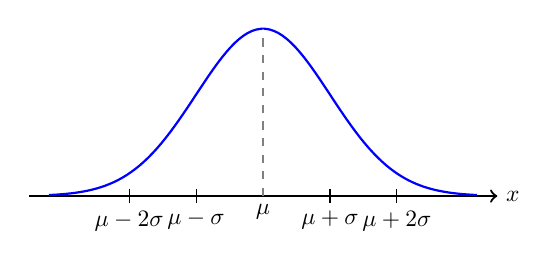
\begin{tikzpicture}[scale=0.85, every node/.style={scale=0.85}]
                % Draw axes
                \draw[->, thick] (-3.5, 0) -- (3.5, 0) node[right] {$x$};
                
                % Draw the bell curve (using a scaled Gaussian function)
                \draw[thick, blue, domain=-3.2:3.2, samples=100] plot (\x, {2.5*exp(-0.5*\x*\x)});
                
                % Center line (Mean)
                \draw[dashed, gray] (0,0) -- (0, 2.5);
                \node[below] at (0,0) {$\mu$};
                
                % Standard Deviation tick marks
                \draw (1, 0.1) -- (1, -0.1) node[below] {$\mu+\sigma$};
                \draw (2, 0.1) -- (2, -0.1) node[below] {$\mu+2\sigma$};
                \draw (-1, 0.1) -- (-1, -0.1) node[below] {$\mu-\sigma$};
                \draw (-2, 0.1) -- (-2, -0.1) node[below] {$\mu-2\sigma$};
            \end{tikzpicture}
        \end{column}
    \end{columns}
\end{frame}

\begin{frame}{The Equation of the Normal Curve}
    The bell shape we just saw is not just a rough sketch; it is defined by a very specific, and slightly intimidating, mathematical formula.

    \begin{definition}[Normal Probability Density Function]
        If a continuous random variable $X$ is normally distributed with mean $\mu$ and standard deviation $\sigma$, its PDF is given by:
        \[ f(x) = \frac{1}{\sigma \sqrt{2\pi}} e^{-\frac{1}{2}\left(\frac{x-\mu}{\sigma}\right)^2} \]
        \textit{for any real number $x$ ($-\infty < x < \infty$).}
    \end{definition}
    
\begin{example}{Question: What is the CDF for the normal curve?}
        How do we integrate the PDF to get the CDF for the normal curve?
    \end{example}

    \only<presentation>{\pause \vspace{0.2cm}}


\end{frame}

\begin{frame}
\frametitle{Integrating the normal distribution}
\begin{solution}
This integral 
\[
\int_{-\infty}^{x} e^{-\frac{1}{2}\left(\frac{x-\mu}{\sigma}\right)^2} \mathrm{d}x
\]
can \emph{only be done numerically}
\end{solution}

\pause

\begin{block}{Why do we use Python (or Tables)?}
        Remember that probability is the \textbf{area} under this curve. However, the integral of this specific function \textbf{cannot be solved algebraically}! There is no closed-form solution. 
        
        We must use numerical approximation (like Python's \texttt{scipy.stats.norm.cdf}) to find the areas.
    \end{block}

    \only<article>{
        \textbf{Engineering Note:} You will not be asked to integrate this function by hand in this course. However, you must recognise its components. Notice how the exponent contains the fraction $\frac{x-\mu}{\sigma}$. This ratio (the distance from the mean, scaled by the standard deviation) is so mathematically important that we give it a special name: the \textbf{Z-score}. We will explore this in the next section.
    }
\end{frame}

\begin{frame}{The CDF and the Error Function ($\text{erf}$)}
    As we saw, the integral for the Normal CDF cannot be solved using standard algebra. To evaluate it, mathematicians defined a special, non-elementary function called the \textbf{Error Function} ($\text{erf}$).

    \begin{definition}[The Error Function]
        \[ \text{erf}(z) = \frac{2}{\sqrt{\pi}} \int_{0}^{z} e^{-t^2} \,dt \]
    \end{definition}

    \pause \only<presentation>{\vspace{0.2cm}}
    The exact Cumulative Distribution Function (CDF) of any Normal Distribution can be expressed using this function:
    \[ F(x) = P(X \leq x) = \frac{1}{2} \left[ 1 + \text{erf}\left( \frac{x-\mu}{\sigma \sqrt{2}} \right) \right] \]

    \only<article>{
        \textbf{Why should an Engineer care?} You will rarely calculate the Error Function by hand—that is exactly why we use \texttt{scipy.stats} in Python. However, you will see $\text{erf}(z)$ (and its close cousin, the Q-function) constantly in your later modules. It is the fundamental equation used in \textbf{Digital Communications} when calculating the Bit Error Rate (BER) of a noisy signal, and in \textbf{Semiconductor Physics} when modelling the diffusion of dopants in silicon.
    }
\end{frame}

\section{Standardisation and Z-Scores}

\begin{frame}{The Infinite Family of Normal Curves}
\only<article>{    Different engineers face different statistical problems. By changing the mean ($\mu$) or the standard deviation ($\sigma$), we create infinitely many different Normal curves.}

    \centering
    \begin{tikzpicture}[scale=1.0, every node/.style={scale=0.9}]
        
        % Declaring the generic Gaussian math function locally for standard TikZ
        \tikzset{declare function={normpdf(\x,\m,\s)=1/(\s*sqrt(2*pi))*exp(-0.5*((\x-\m)/\s)^2);}}

        % --- Drawing the Shared Axes ---
        % Domain needs to cover all three curves, approx -5 to +7
        \draw[->, thick] (-5.5, 0) -- (7.5, 0) node[right] {$x$};
        \draw[->, thick] (0, 0) -- (0, 4.5) node[above] {$f(x)$};
        \node[gray] at (-2, 4) {\textit{Probability Density}};

        % --- Tick Marks ---
        \foreach \x in {-5, -2, 0, 4, 7}
            \draw (\x, 0.1) -- (\x, -0.1) node[below] {\x};

        % --- Curve 1: The "Reference" (Standard Normal-ish) ---
        % N(0, 1^2). Peak height is approx 0.4. Multiplied by 5 for visual scale.
        % Domain needs 3.5 sigma either side: -3.5 to 3.5
        \draw[thick, blue, domain=-3.5:3.5, samples=100] plot (\x, {5 * normpdf(\x, 0, 1)});
        \node[blue, right] at (0.6, 1.6) {\textbf{A}: $N(0, 1^2)$};

        % --- Curve 2: The Shifted Mean (Server Response Time?) ---
        % N(4, 1^2). Peak height same as A. Multiplied by 5.
        % Domain: 4 +/- 3.5 -> 0.5 to 7.5.
        \draw[thick, red, domain=0.5:7.5, samples=100] plot (\x, {5 * normpdf(\x, 3.5, 1)});
        \node[red, right] at (4.5, 1.2) {\textbf{B}: $N(3.5, 1^2)$};

        % --- Curve 3: The Tight Tolerance (Precise Resistor?) ---
        % N(-2, 0.5^2). Peak height doubles to approx 0.8. Multiplied by 5 -> 4.0.
        % Domain: -2 +/- (3.5*0.5) -> -3.75 to -0.25
        \draw[thick, green!70!black, domain=-3.75:-0.25, samples=100] plot (\x, {5 * normpdf(\x, -2, 0.5)});
        \node[green!70!black, left] at (-2.3, 3.5) {\textbf{C}: $N(-2, 0.5^2)$};

    \end{tikzpicture}

    \only<presentation>{
        \begin{center}
            \textbf{A} is centered at 0. \textbf{B} has the same shape, but is shifted. \\
            \textbf{C} is tall and skinny because its standard deviation is small.
        \end{center}
    }
    
    \only<article>{
        \vspace{0.4cm}
        \textbf{Engineering Interpretations:}
        \begin{itemize}
            \item \textbf{Comparing Curves A and B:} These distributions have the \textit{exact same spread} ($\sigma=1$). An error of $+1$ is equally probable on Line A or Line B. The only difference is where the system is centred.
            \item \textbf{Comparing Curves A and C (The Precision Problem):} Curve C has a much smaller standard deviation ($\sigma=0.5$) than Line A. Curve C might represent a very expensive, high-precision laser trimming process. It guarantees almost no variation from its centre. In contrast, Line A is \lq slacker\rq, with much wider engineering tolerances. 
        \end{itemize}
        The fact that these curves are all different is why we use \textbf{Standardisation} (Z-scores) next—to bring them all onto the same playing field.
    }
\end{frame}

\subsection{Z-Scores}
\begin{frame}{Standardising the Normal Curve}
\only<article>{There are infinitely many Normal curves—every time you change the mean ($\mu$) or the standard deviation ($\sigma$), you get a differently shaped bell. }
    
    Before computers existed, engineers couldn't calculate the area under every possible curve. Instead, they used a mathematical trick called \textbf{Standardisation} to convert \textit{any} normal distribution into one single, universal curve.

    \begin{definition}[The Z-Score]
        A Z-score transforms a raw measurement ($X$) into a standardised number by subtracting the mean and dividing by the standard deviation:
        \[ Z = \frac{X - \mu}{\sigma} \]
    \end{definition}

    \only<article>{
        \vspace{0.2cm}
        \textbf{What does Z actually mean?} A Z-score tells you exactly \textbf{how many standard deviations} a specific value is away from the mean. 
        \begin{itemize}
            \item A Z-score of $0$ means the value is exactly on the mean.
            \item A Z-score of $+1.5$ means the value is 1.5 standard deviations above the mean.
            \item A Z-score of $-2.0$ means the value is 2 standard deviations below the mean.
        \end{itemize}
    }
\end{frame}

\subsection{The Standard Normal Distribution}
\begin{frame}{The Standard Normal Distribution}
    When you apply the Z-score formula to every single data point in a dataset, you create a brand new distribution called the \textbf{Standard Normal Distribution}.

    \vspace{0.2cm}
    \begin{block}{Properties of the Standard Normal ($Z$)}
        \begin{itemize}
            \item The mean is always shifted to zero: $\mu_Z = 0$
            \item The standard deviation is always scaled to one: $\sigma_Z = 1$
            \item Notation: $Z \sim N(0, 1)$
        \end{itemize}
    \end{block}

    \pause \vspace{0.2cm}
    \begin{alertblock}{The Golden Rule of Z-Scores}
        The area under the curve for the original $X$ value is \textbf{exactly the same} as the area under the curve for the new $Z$ value. 
        \[ P(X \leq x) = P\left(Z \leq \frac{x - \mu}{\sigma}\right) \]
    \end{alertblock}
\end{frame}

\begin{frame}[allowframebreaks]{Example: Comparing Apples to Oranges}
    Z-scores aren't just an old trick for using lookup tables; they are the ultimate engineering tool for comparing different systems!

    \vspace{0.2cm}
    \begin{example}[Quality Control on Two Lines]
        You are managing two different manufacturing lines.
        \begin{itemize}
            \item \textbf{Line A (Resistors):} $\mu = 1000\,\Omega$, $\sigma = 20\,\Omega$.
            \item \textbf{Line B (Capacitors):} $\mu = 50\,\mu\text{F}$, $\sigma = 0.5\,\mu\text{F}$.
        \end{itemize}
        
        \vspace{0.2cm}
        An inspector pulls one component from each line:
        \begin{itemize}
            \item The resistor measures $1035\,\Omega$.
            \item The capacitor measures $51.2\,\mu\text{F}$.
        \end{itemize}
        
        \structure{Question:} Which of these two components is more \lq unusual\rq\ (i.e., relatively further from its design specification)?
    \end{example}

    \framebreak
    \begin{solution}
    	\small
        We cannot compare Ohms to Microfarads directly. We must convert both to dimensionless (unitless) Z-scores!
        
        \textbf{1. Line A (Resistor):}
        \[ Z_A = \frac{X - \mu}{\sigma} = \frac{1035 - 1000}{20} = \frac{35}{20} = \mathbf{1.75} \]
        The resistor is $1.75$ standard deviations above its mean.
        
        \textbf{2. Line B (Capacitor):}
        \[ Z_B = \frac{X - \mu}{\sigma} = \frac{51.2 - 50}{0.5} = \frac{1.2}{0.5} = \mathbf{2.40} \]
        The capacitor is $2.40$ standard deviations above its mean.
        
        \textbf{Conclusion:} Even though the resistor's absolute error was $35$ and the capacitor's error was only $1.2$, the \textbf{capacitor is much more unusual}. It is further out in the tail of its distribution!
    \end{solution}
\end{frame}

\subsection{The Standard Normal Table ($Z$-Table)}
\begin{frame}{The Standard Normal Table ($Z$-Table)}
    \only<article>{Look up the first decimal place on the left, and the second decimal place across the top. The intersection is the cumulative area $P(Z \leq z)$.}
\begin{center}
    % On the slides: Maximize vertical space to fill the screen
    \only<presentation>{
        \includegraphics[trim=2cm 2.5cm 2cm 8.25cm, clip, height=0.95\textheight, keepaspectratio]{Resources/NormalDistibutionTable.pdf}
    }
    % In the handout: Constrain by width so it sits nicely within the page margins
    \only<article>{
        \includegraphics[trim=2cm 2.5cm 2cm 8.25cm, clip, width=0.85\textwidth, keepaspectratio]{Resources/NormalDistibutionTable.pdf}
    }
\end{center}
    
\end{frame}

\begin{frame}{How to Read a Z-Table}
   \only<article>{ Before Python, engineers relied on printed \textbf{Standard Normal Tables} (which you have as a handout). This table gives the cumulative probability $\Phi(z) = P(Z \leq z)$.}

    \begin{block}{Reading the Table}
        \begin{itemize}
            \item \textbf{Left Column:} Gives the $Z$-score up to the first decimal place (e.g., $1.2$).
            \item \textbf{Top Row:} Gives the second decimal place (e.g., $0.04$).
            \item \textbf{Intersection:} The value at row $1.2$ and column $0.04$ gives the total area: $P(Z \leq 1.24)$.
            \item \textbf{CP:} The value is 0.8925.
        \end{itemize}
    \end{block}

    \pause \vspace{0.2cm}
    \begin{alertblock}{Handling Negative Z-Scores}
        Notice your table only shows positive $Z$ values. Because the Normal Curve is perfectly symmetric, the left tail is identical to the right tail. To find negative areas, we use the complement rule:
        $$P(Z \leq -z) = 1 - P(Z \leq z)$$
    \end{alertblock}
\end{frame}

\begin{frame}{Worked Example: Calculating Probabilities}
    \begin{example}[Resistor Manufacturing]
        A production line manufactures resistors with a mean resistance of $\mu = 1000\,\Omega$ and a standard deviation of $\sigma = 20\,\Omega$. 
        
        \vspace{0.2cm}
        Assume the resistance values are normally distributed. Using your Z-table handout, calculate:
        \begin{enumerate}
            \item The probability that a randomly selected resistor is \textbf{less than} $1035\,\Omega$.
            \item The probability that a resistor is \textbf{greater than} $1025\,\Omega$.
            \item The probability that a resistor is \textbf{less than} $970\,\Omega$.
        \end{enumerate}
    \end{example}
\end{frame}

\begin{frame}{Solution: Using the Z-Table (1/2)}
    \begin{solution}
        \textbf{1. Less than $1035\,\Omega$:}
        \begin{itemize}
            \item Find the Z-score: $Z = \frac{1035 - 1000}{20} = 1.75$
            \item We want $P(Z \leq 1.75)$. This is a direct lookup.
            \item Look at row \textbf{1.7}, column \textbf{0.05}.
            \item Table value: $\mathbf{0.9599}$ (or 95.99\%).
        \end{itemize}
        
        \pause \vspace{0.3cm}
        \textbf{2. Greater than $1025\,\Omega$:}
        \begin{itemize}
            \item Find the Z-score: $Z = \frac{1025 - 1000}{20} = 1.25$
            \item We want $P(Z > 1.25)$. The table only gives \lq less than\rq\ areas!
            \item Use the complement: $P(Z > 1.25) = 1 - P(Z \leq 1.25)$.
            \item Look at row \textbf{1.2}, column \textbf{0.05}. Table value is $0.8944$.
            \item Answer: $1 - 0.8944 = \mathbf{0.1056}$ (or 10.56\%).
        \end{itemize}
    \end{solution}
\end{frame}

\begin{frame}{Solution: Using the Z-Table (2/2)}
    \begin{solutioncont}
        \textbf{3. Less than $970\,\Omega$:}
        \begin{itemize}
            \item Find the Z-score: $Z = \frac{970 - 1000}{20} = \frac{-30}{20} = -1.50$
            \item We want $P(Z \leq -1.50)$. Our table has no negative numbers!
            \item By symmetry, the extreme left tail area equals the extreme right tail area: \\
                  $P(Z \leq -1.50) = P(Z \geq 1.50) = 1 - P(Z \leq 1.50)$
            \item Look at row \textbf{1.5}, column \textbf{0.00}. Table value is $0.9332$.
            \item Answer: $1 - 0.9332 = \mathbf{0.0668}$ (or 6.68\%).
        \end{itemize}
    \end{solutioncont}
    
    \only<article>{
        \textbf{Tip:} It can be useful, especially when you first start this type of questions, to draw a quick sketch of the bell curve for these problems. Shading the area you are looking for is the single best way to avoid accidentally forgetting the \lq$1 - $\rq\ step for \lq greater than\rq\ or negative Z-score problems.
    }
\end{frame}



\begin{frame}{The Empirical Rule (68-95-99.7)}
    \only<article>{Because the Normal Distribution is universally symmetric, we can use a powerful shortcut to estimate probabilities without doing any calculus!}

    For \textit{any} Normal Distribution:
    \begin{itemize}
        \item \textbf{$\approx 68\%$} of the data falls within \textbf{1 standard deviation} of the mean ($\mu \pm 1\sigma$).
        \item \textbf{$\approx 95\%$} of the data falls within \textbf{2 standard deviations} of the mean ($\mu \pm 2\sigma$).
        \item \textbf{$\approx 99.7\%$} of the data falls within \textbf{3 standard deviations} of the mean ($\mu \pm 3\sigma$).
    \end{itemize}
    
    \only<article>{
        \vspace{0.3cm}
        \textbf{Why this matters to EEEs:} If a manufacturer states that a component's specs are \lq guaranteed to $3\sigma$\rq, they are telling you that 99.7\% of the components will operate within the stated tolerance. Only 3 in 1,000 will fail. This is the foundation of the famous \lq Six Sigma\rq\ quality control methodology.
    }
\end{frame}


\begin{frame}{Example: The Empirical Rule}
    \begin{example}[Manufacturing Tolerances]
        A factory produces 9V batteries. The actual voltage is normally distributed with a mean of $\mu = 9.0\text{V}$ and a standard deviation of $\sigma = 0.1\text{V}$.
        
        \vspace{0.2cm}
        \structure{Questions:}
        \begin{enumerate}
            \item What percentage of batteries will have a voltage between $8.9\text{V}$ and $9.1\text{V}$?
            \item What percentage of batteries will have a voltage between $8.8\text{V}$ and $9.2\text{V}$?
            \item If the battery is considered \lq defective\rq\ if it falls outside of the $8.7\text{V}$ to $9.3\text{V}$ range, what is the defect rate?
        \end{enumerate}
    \end{example}
\end{frame}

\begin{frame}{Solution: The Empirical Rule}
    \begin{solution}
        \begin{enumerate}
            \item $8.9\text{V}$ to $9.1\text{V}$ is exactly $\mu - 1\sigma$ to $\mu + 1\sigma$. \\
            According to the rule, this covers \textbf{$\approx 68\%$} of the batteries.
            
            \vspace{0.3cm}
            \item $8.8\text{V}$ to $9.2\text{V}$ is exactly $\mu - 2\sigma$ to $\mu + 2\sigma$. \\
            This covers \textbf{$\approx 95\%$} of the batteries.
            
            \vspace{0.3cm}
            \item $8.7\text{V}$ to $9.3\text{V}$ represents the $\pm 3\sigma$ range. \\
            We know $\approx 99.7\%$ of batteries fall \textit{inside} this safe range. \\
            Therefore, the defect rate is everything \textit{outside} this range: \\
            $100\% - 99.7\% = \mathbf{0.3\%}$ \textbf{defect rate}.
        \end{enumerate}
    \end{solution}
\end{frame}

\begin{frame}[fragile]{Python: The Normal Distribution}
  \only<article>{  In the old days, engineers had to use massive printed lookup tables to find areas under the Normal curve. Today, we just use the \texttt{scipy.stats} library.


    Because the probability of an exact point is zero, we almost never use the Probability Density Function (\texttt{pdf}) to find probabilities. Instead, we use the Cumulative Distribution Function (\texttt{cdf}) to find areas.

}
    \structure{Solving the Battery Problem ($8.8\text{V}$ to $9.2\text{V}$):}
    \only<article>{To find the area between two points, we calculate the CDF of the upper limit and subtract the CDF of the lower limit.}

    \insertcode{Normal Distribution in Python}{code/NormalDistribution.py}

    \only<article>{
        \vspace{0.2cm}
        \textit{Note: In Python's \texttt{scipy.stats.norm}, the mean $\mu$ is called \texttt{loc} (location) and the standard deviation $\sigma$ is called \texttt{scale}.}
    }
\end{frame}

\subsection{The Grand Convergence: Large Numbers}
\begin{frame}{The Grand Convergence: Large Numbers}
    What happens to our discrete distributions when we deal with massive quantities (like millions of transistors or network packets)? 

   \only<article>{
    As the numbers grow, the \lq blocky\rq\ discrete histograms stretch and smooth out, eventually becoming perfectly bell-shaped.}

    \vspace{0.2cm}
    \begin{columns}[T]
        \begin{column}{0.5\textwidth}
            \begin{block}{Binomial to Normal}
                When $n$ is very large:\\
                $X \sim \text{Bin}(n, p) \approx N(np, np(1-p))$
                
                \vspace{0.1cm}
                \textbf{Parameters:}
                \begin{itemize}
                    \item $\mu = np$
                    \item $\sigma^2 = np(1-p)$
                \end{itemize}
                \vspace{0.1cm}
                \textit{Rule of thumb: $np > 5$ and $n(1-p) > 5$}
            \end{block}
        \end{column}
        
        \begin{column}{0.5\textwidth}
            \begin{block}{Poisson to Normal}
                When the rate $\lambda$ is very large:\\
                $X \sim \text{Pois}(\lambda) \approx N(\lambda, \lambda)$
                
                \vspace{0.1cm}
                \textbf{Parameters:}
                \begin{itemize}
                    \item $\mu = \lambda$
                    \item $\sigma^2 = \lambda$
                \end{itemize}
                \vspace{0.1cm}
                \textit{Rule of thumb: $\lambda > 20$}
            \end{block}
        \end{column}
    \end{columns}

    \only<article>{
        \vspace{0.3cm}
        \textbf{Why do engineers do this?} Try calculating the exact Binomial probability of 5,000 successes out of 10,000 trials. The formula requires $10000!$, which will instantly crash most calculators and overflow standard computer memory limits. By approximating it with the Normal Distribution, the math becomes instantly solvable using the Z-scores and lookup tables we just learned!
    }
\end{frame}

\subsection{Example: Binomial to Normal}
\begin{frame}[allowframebreaks]{Example: Binomial to Normal}
    \begin{example}[Manufacturing Yield]
        A factory produces memory chips with a historical defect rate of 20\% ($p = 0.2$). Today, they manufactured $400$ chips. 
        
        Using the Normal approximation, what is the probability that they produced \textbf{less than 64} defective chips?
        
        Comment on the how your would do the exact calculation?
    \end{example}

    \pause
    \begin{solution}
        \textbf{Step 1: Check the rules and find the parameters.}
        \begin{itemize}
            \item Check: $np = 400 \times 0.2 = 80$ (Greater than 5! \checkmark)
            \item Mean: $\mu = np = 80$ defects.
            \item Variance: $\sigma^2 = np(1-p) = 80 \times 0.8 = 64$.
            \item Standard Deviation: $\sigma = \sqrt{64} = \mathbf{8}$ defects.
        \end{itemize}
        
        \vspace{0.2cm}
        \textbf{Step 2: Convert to a Z-score.}
        We want $P(X < 64)$.
        \[ Z = \frac{X - \mu}{\sigma} = \frac{64 - 80}{8} = \frac{-16}{8} = \mathbf{-2.00} \]
        
        \vspace{0.2cm}
        \textbf{Step 3: Look up the area.}
        Using our symmetric Z-table: $P(Z < -2.00) = 1 - P(Z \leq 2.00)$. \\
        Table lookup for $2.00$ is $0.9772$. \\
        Answer: $1 - 0.9772 = \mathbf{0.0228}$ \textbf{(or 2.28\%)}.
    \end{solution}
\end{frame}

\begin{frame}
\begin{solution}
   \textbf{Step 4: The Reality Check (Exact vs. Approx)} \\
        If we asked a computer to calculate the exact, discrete Binomial probability, it would have to sum 64 massive factorial calculations:
        \[ P(X < 64) = P(X \leq 63) = \sum_{x=0}^{63} \binom{400}{x} (0.2)^x (0.8)^{400-x} = \mathbf{0.0195} \text{ \textbf{(1.95\%)}} \]
        
        \vspace{0.1cm}
        \begin{block}{Comparison}
            Our quick Normal approximation ($2.28\%$) is very close to the exact value ($1.95\%$), but it is off by about $0.33\%$. 
            
            \textit{Note: If we apply a $\pm 0.5$ Continuity Correction and look up $P(X < 63.5)$ instead, our Z-score becomes $-2.06$, giving an approximation of \textbf{1.97\%}—an almost perfect match!}
        \end{block}
    \end{solution}


\end{frame}

\subsection{Visualising the Convergence}
\begin{frame}{Visualising the Convergence}
    \only<article>{
        Let return to our coin flip case. Here is the visual proof of the Grand Convergence. We are plotting the exact Binomial probability of getting heads (bars) overlaid with the Normal approximation (the red curve) for $n=10$, $n=100$, and $n=1000$ flips.
        
        \vspace{0.5cm}
        \noindent
        % Minipages guarantee side-by-side layout in Article mode
        \begin{minipage}[t]{0.31\textwidth}
            \centering
            \textbf{$n = 10$ flips} \\
            \vspace{0.2cm}
            \includegraphics[width=\textwidth]{Resources/Convergence_n10.pdf}
            
            \vspace{0.1cm}
            \footnotesize The Binomial bars are wide and \lq blocky\rq. The Normal curve is a decent fit, but the gaps are visible.
        \end{minipage}%
        \hfill
        \begin{minipage}[t]{0.31\textwidth}
            \centering
            \textbf{$n = 100$ flips} \\
            \vspace{0.2cm}
            \includegraphics[width=\textwidth]{Resources/Convergence_n100.pdf}
            
            \vspace{0.1cm}
            \footnotesize The discrete bars are getting thinner. The Normal curve now traces them almost perfectly.
        \end{minipage}%
        \hfill
        \begin{minipage}[t]{0.31\textwidth}
            \centering
            \textbf{$n = 1000$ flips} \\
            \vspace{0.2cm}
            \includegraphics[width=\textwidth]{Resources/Convergence_n1000.pdf}
            
            \vspace{0.1cm}
            \footnotesize The discrete histogram has become so dense it is indistinguishable from the continuous Normal curve.
        \end{minipage}
        
        \vspace{0.5cm}
        \textbf{The Takeaway:} This is why we can swap a complex discrete summation for a simple continuous integral when working with large numbers. The error between the two models shrinks to near zero.
    }
    
    \only<presentation>{
        \begin{columns}[T]
            % Column 1: n = 10
            \begin{column}{0.33\textwidth}
                \centering
                \textbf{$n = 10$ flips} \\
                \vspace{0.2cm}
                \includegraphics[width=\textwidth]{Resources/Convergence_n10.pdf}
                
                \vspace{0.1cm}
                \scriptsize The Binomial bars are wide and \lq blocky\rq. The Normal curve is a decent fit, but the gaps are visible.
            \end{column}
            
            % Column 2: n = 100
            \begin{column}{0.33\textwidth}
                \centering
                \textbf{$n = 100$ flips} \\
                \vspace{0.2cm}
                \includegraphics[width=\textwidth]{Resources/Convergence_n100.pdf}
                
                \vspace{0.1cm}
                \scriptsize The discrete bars are getting thinner. The Normal curve now traces them almost perfectly.
            \end{column}
            
            % Column 3: n = 1000
            \begin{column}{0.33\textwidth}
                \centering
                \textbf{$n = 1000$ flips} \\
                \vspace{0.2cm}
                \includegraphics[width=\textwidth]{Resources/Convergence_n1000.pdf}
                
                \vspace{0.1cm}
                \scriptsize The discrete histogram has become so dense it is indistinguishable from the continuous Normal curve!
            \end{column}
        \end{columns}
    }
\end{frame}

\subsection{Example: Poisson to Normal}
\begin{frame}[allowframebreaks]{Example: Poisson to Normal}
    \begin{example}[Fiber Optic Packets]
        A fibre optic router receives an average of $100$ data packets per millisecond ($\lambda = 100$). 
        
        Using the Normal approximation, what is the probability that the router receives \textbf{more than 120} packets in the next millisecond?
        
        Comment of how you would do the exact calculation?
    \end{example}

    \pause
    \begin{solution}
        \textbf{Step 1: Check the rules and find the parameters.}
        \begin{itemize}
            \item Check: $\lambda = 100$ (Greater than 20! \checkmark)
            \item Mean: $\mu = \lambda = 100$ packets.
            \item Variance: $\sigma^2 = \lambda = 100$.
            \item Standard Deviation: $\sigma = \sqrt{100} = \mathbf{10}$ packets.
        \end{itemize}
        
        \vspace{0.2cm}
        \textbf{Step 2: Convert to a Z-score.}
        We want $P(X > 120)$.
        \[ Z = \frac{X - \mu}{\sigma} = \frac{120 - 100}{10} = \frac{20}{10} = \mathbf{2.00} \]
        
       \end{solution}

\end{frame}

\begin{frame}
\begin{solutioncont}
        \textbf{Step 3: Look up the area.}
        Because we want \lq more than\rq , we use the complement rule: \\
        $P(Z > 2.00) = 1 - P(Z \leq 2.00)$. \\
        Table lookup for $2.00$ is $0.9772$. \\
        Answer: $1 - 0.9772 = \mathbf{0.0228}$ \textbf{(or 2.28\%)}.
        
         \textbf{Step 4: The Reality Check (Exact vs. Approx)} \\
       \only<article>{ If we asked a computer to evaluate the exact discrete Poisson formula, it would sum the probabilities of every integer from $0$ to $120$ and subtract from $1$:}
        \[ P(X > 120) = 1 - \sum_{x=0}^{120} \frac{e^{-100} 100^x}{x!} = \mathbf{0.0227} \text{ \textbf{(2.27\%)}} \]
        
        \begin{block}{Comparison}
            Our hand-calculated Normal approximation ($2.28\%$) is accurate to the exact Poisson value ($2.27\%$) to within one-hundredth of a percent! The approximation performs incredibly well when $\lambda$ is large.
        \end{block}
    \end{solutioncont}

    \only<article>{
       \subsubsection{Continuity Correction} 
       
       Technically, when mapping a \lq chunky\rq\ discrete histogram onto a smooth continuous curve, we should use a \textbf{Continuity Correction} (e.g., checking $X < 63.5$ instead of $X < 64$ to account for the width of the histogram bin). However, when $n$ and $\lambda$ are very large, this correction factor becomes so infinitesimally small that engineers often ignore it for rough approximations. For this introductory level, we are omitting the $\pm 0.5$ correction to focus squarely on the Z-score mechanics.
    }
\end{frame}

\section{Beyond the Normal Curve}
\begin{frame}{Beyond the Normal Curve}
    The Normal distribution is everywhere, but it is not the only continuous probability model. Depending on your engineering discipline, you will eventually encounter others:

    \vspace{0.2cm}
    \begin{itemize}
        \item \textbf{Uniform Distribution:} A flat rectangle where any value in a range is equally likely. 
        \begin{itemize}
            \item \textit{Used in:} Modelling quantisation error in Analog-to-Digital Converters (ADCs).
        \end{itemize}
        
        \vspace{0.2cm}
        \item \textbf{Exponential Distribution:} Models the time between independent events.
        \begin{itemize}
            \item \textit{Used in:} Reliability engineering (Mean Time Between Failures) and network queueing delays.
        \end{itemize}
        
        \vspace{0.2cm}
        \item \textbf{Weibull \& Rayleigh Distributions:} Skewed distributions that model asymmetric continuous data.
        \begin{itemize}
            \item \textit{Used in:} Predicting material fatigue life in mechanical engineering, or modeling wireless signal fading in communications.
        \end{itemize}
    \end{itemize}

    \only<article>{
        \vspace{0.3cm}
        \textit{Here we will not do into a full details, this is purely to show you that the exact same mechanics they just learned (integrating the PDF to find the CDF and the mean) apply perfectly to all of these advanced distributions.}
    }
\end{frame}

\subsection{Formulas for Other Distributions}
\begin{frame}[allowframebreaks]{Formulas for Other Distributions}
    While not part of this course, here is the mathematical reference for the distributions we just mentioned. Notice how every single one still has a clearly defined PDF, mean, and variance.

    \vspace{0.2cm}
    \begin{block}{Continuous Uniform Distribution: $U(a, b)$}
        Models an equal probability across a specific range from $a$ to $b$.
        \begin{itemize}
            \item \textbf{PDF:} $f(x) = \frac{1}{b-a} \quad \text{for } a \leq x \leq b$
            \item \textbf{Mean:} $\mu = \frac{a+b}{2}$
            \item \textbf{Variance:} $\sigma^2 = \frac{(b-a)^2}{12}$
        \end{itemize}
    \end{block}

    \vspace{0.2cm}
    \begin{block}{Exponential Distribution: $\text{Exp}(\lambda)$}
        Models the time between events, using a rate parameter $\lambda$.
        \begin{itemize}
            \item \textbf{PDF:} $f(x) = \lambda e^{-\lambda x} \quad \text{for } x \geq 0$
            \item \textbf{Mean:} $\mu = \frac{1}{\lambda}$
            \item \textbf{Variance:} $\sigma^2 = \frac{1}{\lambda^2}$
        \end{itemize}
    \end{block}

    \framebreak

    \begin{block}{Rayleigh Distribution}
        Models the overall magnitude of a vector when its components are independent and normally distributed (like 2D wind velocity or radio signal scattering).
        \begin{itemize}
            \item \textbf{PDF:} $f(x) = \frac{x}{\sigma^2} e^{-x^2 / (2\sigma^2)} \quad \text{for } x \geq 0$
            \item \textbf{Mean:} $\mu = \sigma \sqrt{\frac{\pi}{2}}$
            \item \textbf{Variance:} $V(X) = \frac{4-\pi}{2}\sigma^2$
        \end{itemize}
    \end{block}

    \vspace{0.2cm}
    \begin{block}{Weibull Distribution (2-Parameter)}
        A highly versatile distribution heavily used in reliability engineering, featuring a shape parameter $k$ and a scale parameter $\lambda$.
        \begin{itemize}
            \item \textbf{PDF:} $f(x) = \frac{k}{\lambda} \left(\frac{x}{\lambda}\right)^{k-1} e^{-(x/\lambda)^k} \quad \text{for } x \geq 0$
            \item \textbf{Mean:} $\mu = \lambda \Gamma\left(1 + \frac{1}{k}\right)$
            \item \textit{Note: $\Gamma$ represents the Gamma function. The exact variance involves multiple Gamma terms!}
        \end{itemize}
    \end{block}
\end{frame}

\section{Summary: Continuous Probability Distributions}
\begin{frame}{Summary: Continuous Probability Distributions}
    \begin{itemize}
        \item \textbf{Continuous Random Variables:}
        \begin{itemize}
            \item Used for continuous physical measurements (voltage, resistance, time).
            \item Probability is \textbf{Area}: $P(a \leq X \leq b) = \int_{a}^{b} f(x) \dd x$.
            \item The probability of measuring an \textit{exact} point is always zero.
            \item The CDF, $F(x)$, gives the accumulated probability up to $x$.
        \end{itemize}
        
        \item \textbf{The Normal Distribution \& Z-Scores:}
        \begin{itemize}
            \item The fundamental symmetric bell curve: $X \sim N(\mu, \sigma^2)$.
            \item \textbf{Standardisation:} We can compare entirely different systems by converting raw values to unitless Z-scores: $Z = \frac{X - \mu}{\sigma}$.
            \item A Z-score tells you exactly how many standard deviations a value is from the mean.
            \item \textbf{Empirical Rule:} 68\% ($1\sigma$), 95\% ($2\sigma$), and 99.7\% ($3\sigma$).
        \end{itemize}
        
        \item \textbf{The Grand Convergence:}
        \begin{itemize}
\item At large scales, Binomial and Poisson distributions can be approximated by the Normal curve.
        \end{itemize}
    \end{itemize}
\end{frame}

\only<article>{
\section{Exercise Questions}
%!TEX root = ExerciseSheet2.tex
% -----------------------------------------------------------------------------
% PART A
% -----------------------------------------------------------------------------

\subsection*{Part A: The Idea}
\textit{These questions test the mathematical definitions and calculations devoid of physical context.}

\begin{enumerate}[label=\textbf{Q\arabic*.}, leftmargin=*]
    \item \textbf{Continuous Random Variables \& Probability Density Functions} \\
    A continuous random variable $X$ has the following Probability Density Function (PDF):
    $$
    f(x) = \begin{cases} 
    cx^2 & \text{for } 0 \leq x \leq 3 \\ 
    0 & \text{otherwise} 
    \end{cases}
    $$
    \begin{enumerate}[label=\arabic*.]
        \item Find the value of $c$, knowing that the total area under a valid PDF must equal 1.
        \item Calculate the probability $P(X \leq 2)$ by integrating the PDF.
        \item Calculate the expected value, $E(X)$.
    \end{enumerate}
    \vspace{0.3cm}

    \item \textbf{The Standard Normal Distribution ($Z$)} \\
    Let $Z$ be a standard normal random variable, $Z \sim N(0, 1^2)$. Using your standard normal distribution tables, find the following probabilities:
    \begin{enumerate}[label=\arabic*.]
        \item $P(Z \leq 1.25)$
        \item $P(Z > 0.50)$ \textit{(Hint: Use the complement rule).}
        \item $P(Z \leq -1.10)$ \textit{(Hint: Use the symmetry of the normal curve).}
    \end{enumerate}
    \vspace{0.3cm}

    \item \textbf{Standardisation \& The Normal Distribution} \\
    Let $X$ be a normally distributed random variable, $X \sim N(\mu=50, \sigma^2=16)$. Note that the standard deviation is $\sigma = 4$.
    \begin{enumerate}[label=\arabic*.]
        \item Calculate the Z-score for $x = 56$.
        \item Calculate the Z-score for $x = 42$.
        \item Find the probability $P(X \leq 56)$ by converting it to a Z-score and using the standard normal table.
    \end{enumerate}

\end{enumerate}

\vspace{0.8cm}

% -----------------------------------------------------------------------------
% PART B
% -----------------------------------------------------------------------------
\subsection*{Part B: Exam style questions: Engineering Application}
\textit{These questions test the exact same mathematical concepts as Part A, but applied to the Electrical Engineering scenarios discussed in the lecture.}

\begin{enumerate}[label=\textbf{Q\arabic*.}, leftmargin=*, start=4]

    \item \textbf{Continuous PDFs in Engineering (Sensor Drift)} \\
    An engineer models the voltage drift $X$ (in millivolts) of a thermal sensor prototype using the continuous PDF:
    $$
    f(x) = \begin{cases} 
    0.5x & \text{for } 0 \leq x \leq 2 \\ 
    0 & \text{otherwise} 
    \end{cases}
    $$
    \begin{enumerate}[label=\arabic*.]
        \item Calculate the probability that the sensor drift is \textbf{less than 1mV} (i.e., $P(X < 1)$).
        \item Calculate the expected average voltage drift, $E(X)$.
        \item Determine the Cumulative Distribution Function (CDF), $F(x)$, by integrating from $0$ to $x$.
    \end{enumerate}
    \vspace{0.3cm}

    \item \textbf{Normal Quality Assurance (Manufacturing Tolerances)} \\
    A production line manufactures precision resistors. The resistance values are normally distributed with a mean of $1000\,\Omega$ ($\mu = 1000$) and a standard deviation of $20\,\Omega$ ($\sigma = 20$).
    \begin{enumerate}[label=\arabic*.]
        \item What is the probability that a randomly selected resistor has a resistance of \textbf{less than $1035\,\Omega$}?
        \item What is the probability that a resistor has a resistance \textbf{greater than $1025\,\Omega$}?
        \item The manufacturer guarantees that any resistor outside the range of $960\,\Omega$ to $1040\,\Omega$ will be rejected. Using the Empirical Rule (68-95-99.7), what percentage of resistors are expected to be \textbf{accepted}?
    \end{enumerate}
    \vspace{0.3cm}

    \item \textbf{Comparing Components (Z-Scores in Action)} \\
    You are sourcing components from two different suppliers. You test one component from each:
    \begin{itemize}
        \item \textbf{Supplier A (Capacitors):} $\mu = 50\,\mu\text{F}$, $\sigma = 0.5\,\mu\text{F}$. The tested capacitor measures $51.2\,\mu\text{F}$.
        \item \textbf{Supplier B (Inductors):} $\mu = 100\text{ mH}$, $\sigma = 2\text{ mH}$. The tested inductor measures $104\text{ mH}$.
    \end{itemize}
    \begin{enumerate}[label=\arabic*.]
        \item Calculate the unitless Z-score for the tested capacitor.
        \item Calculate the unitless Z-score for the tested inductor.
        \item Mathematically, which of these two components is more \lq unusual\rq\ (i.e., relatively further from its design specification)?
    \end{enumerate}
    \vspace{0.3cm}

    \item \textbf{The Grand Convergence (Normal Approximation)} \\
    A factory produces memory chips with a historical defect rate of $20\%$ ($p = 0.2$). Today, they manufactured a massive batch of $400$ chips ($n = 400$). Calculating the exact Binomial probability of failures would overload a standard calculator.
    \begin{enumerate}[label=\arabic*.]
        \item Calculate the expected mean ($\mu$) and standard deviation ($\sigma$) of the defects to build our continuous Normal approximation.
        \item Using your Normal approximation parameters, calculate the Z-score for finding exactly $64$ defective chips.
        \item Use the Z-table to find the approximate probability that the factory produced \textbf{less than 64} defective chips today.
    \end{enumerate}

\end{enumerate}


}

     